\section{Overview}
 
% main topic sentence for each paragraph

% 우리는 코드 변환을 기반을 기존의 모델을 자동으로 분산화하는 기법을 제안한다.
We propose the code transformation-based approach 
for automated distributed training of TensorFlow DL models.
As explained in the previous section, distributing TensorFlow DL models
with Horovod library requires adding and editing the origianl codes.
Currently, the developers must fully understand the model codes and
manually rewrite the model codes.
This also includes understanding the Horovod library usage by reading
the library documentation and code exmaples.
To ease the burden of the rewriting process, 
we utilize the code transformation technique to automatically rewrite the
input TensorFlow model code with Horovod library APIs.

% 기존의 모델에 적용하는 코드 변환 규칙을 정의하기 위해 horovod 라이브러리 문서와
% 코드 예제를 검토했다. 그 결과로 TF 모델을 4가지로 분류하고 각 분류에 맞는
% 변환 규칙을 정의할 수 있었다.
To define the code transformation rule for distributing TensorFlow DL models,
we manually inspected the Horovod library documentation and code examples.
In this end, we identified four categories of TensorFlow DL models.
We define four \textit{training API patterns}, which are common code patterns of 
TensorFlow APIs appearing in the TensorFlow DL model.
To categorize the TensorFlow DL models into one of the four paterns, 
we implemented the training API pattern identifier. 
In this process, we identified that the pattern identifier must know the  
class inheritance relationship between TensorFlow library classes and
user-defined classes.
To solve this problem, we also implemented the class hierarchy analyzer to
retrive the class inheritance information of the TensorFlow DL models.

\begin{figure}[ht!]
  \centering
  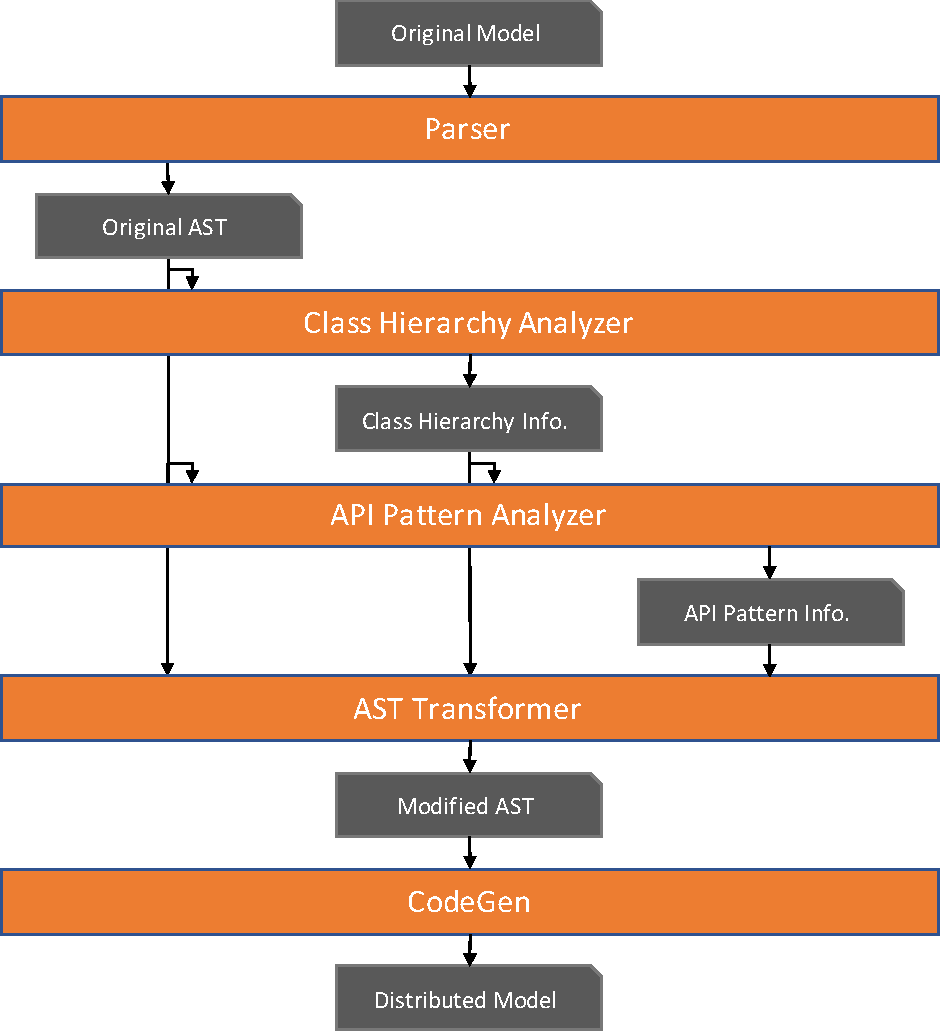
\includegraphics[width=0.5\textwidth]{tool-arch.pdf}
  \caption{Overall structure of the 
  automated transformation for distributed training}
  \label{sysarch}
\end{figure}

% 우리 기법은 입력으로 주어진 TF 모델에서 먼저 API 패턴을 인식하고
% 해당 패턴에 맞는 코드 변환 규칙을 적용하는 방식으로 작동한다.
% 이를 위해 설계한 우리 기법의 overview는 피규어와 같다...
Our approach first analyzes the class hierarchy of the input model then
identify the training API pattern of the model.
Then the code transformer selects the correct transformation rule according
to the training API pattern then applies the rule to get the distributed
model as an output.
Figure \ref{sysarch} illustrates the overview of our appraoch.

\textbf{Parser}
Parser parses input Python code package
into the set of ASTs.
We assume that the input single-GPU-based model is given as a Python code
package that resides in a single file directory.
Given the directory, the parser module first parses all Python code files
in the package to ASTs.
The Python abstract syntax and details on the parser implementation
are described in section \ref{sec:pysyn}.

\textbf{Class Hierarchy Analyzer}
Class hierarchy analyzer analyzes the class inheritance relation
between user-defined classes and TensorFlow library classes and
outputs the class hierarchy graph.
We implemented the class hierarchy analysis
for Python codes as the class hierarchy analyzer module.
The class hierarchy analyzer produces the class hierarchy graph
for the model package and returns it to the API pattern analyzer and 
AST transformer modules. The details of the class hierarchy analyzer are
described in section \ref{sec:cha}.

\textbf{Training API Pattern Identifier}
Training API pattern identifier 
indentifies the TensorFlow training APIs used in the training code AST
and returns the training API pattern for the code.
The details of the training API pattern identifier described 
in section \ref{sec:pattern}.

\textbf{AST Transformer}
AST transformer module applies the correct transformation to the
training code AST to retain the distributed training code AST.
To select the correct transformation rule,
the AST transformer utlizes the class hierarchy information and
the training API pattern informatino.
We defined formal transformation rules which are composed of
\textit{transform functions} from ASTs to ASTs.
By applying the transform function to the input AST,
the AST transformer module outputs the transformed AST as an output.
The details of the AST transformer is described in section \ref{sec:trans}
